%!TEX root = paper.tex


\section{Data Collection Methodology}
\label{sec:bluetana}

Driven by the observation that skimmers are hard to find---few pumps in San Diego, Arizona, and Florida have been found to have 
skimmers installed in them (Table~\ref{tab:wildskims})---we created a tool, called Bluetana, to evaluate the
effectiveness of Bluetooth-based skimmer detection.
%
We begin by presenting an overview of the tool and the data it collects.
%
Then we describe how Bluetana identifies suspicious devices and directs users
to collect additional data.
%
Finally, we discuss how we retroactively inspect data to find skimmers. 

\subsection{Crowdsourcing Bluetooth Scanning}
\label{sec:bluetana:tool}

We developed Bluetana, an Android-based measurement tool that officials and volunteers
use to scan for skimmers at gas stations.
%
%is an Android application that is provided to
%
Bluetana scans for nearby Bluetooth---both Classic and Bluetooth Low
Energy (BLE)---devices every 5~seconds using Android's Bluetooth API.
%
It collects the Bluetooth scans and geo-location data, and uploads this data to a
secure database over a cellular link.
%
Bluetana collects all of the Bluetooth scan data that Android makes available, including
Device name, MAC Address, Class-of-Device\footnote{Class-of-Device is twenty
  four bits indicating the device's intended use, such as \emph{smartphone} or
  \emph{speaker}.}, and signal strength (RSSI).

\paragraph{How we visited 1200 gas stations}
%
We outfitted ~\numvolunteers~ volunteers and inspectors in six U.S. states (CA, AZ, MD, NC,
NV, IL) with low-end smartphones running Bluetana in kiosk mode (they could not
close the application).
%
We selected officials who frequent gas stations as part of their daily job
duties. Primarily, they were Weights and Measures inspectors.
%Periodically, the application automatically transmits them over the cellular
%link to our secure database.
%
%It also records the device's geo-location during the scan when it completes. 

\subsubsection*{Indicating suspicious devices to inspire data collection}

\begin{figure}
\centering
\captionsetup{justification=centering}
\includegraphics[width=0.8\linewidth]{skimmer/fig/bluetana_screenshot}
\caption{
\label{fig:bluetana}
The Bluetana user interface. Bluetana highlights suspicious devices, inspiring users to collect more
signal strength samples, and even perform inspections.
}
\end{figure}



The Bluetana display shows a list of Bluetooth devices detected during scanning.
%
When Bluetana detects a potential skimmer, it indicates this to the user by
highlighting the device record (Figure~\ref{fig:bluetana}).
%
The Bluetooth scan profile of the modules that have been found in skimmers inform which devices we highlight in Bluetana.
 
Skimmers recovered by LE are often found to use CSR (Qualcomm) chip-set-based Bluetooth modules.
%, and criminals
%tend to leave the Bluetooth properties of these modules at their factory defaults.
%
Our highlighting procedure primarily looks for the default Bluetooth profile of
these modules---with the exception of the Device Name which can be missing due to poor
signal strength, and modified by criminals in an attempt to hide the device (Section~\ref{sec:bluetooth}).
%
The factory default Bluetooth scan profile (i.e., MAC prefix, Device Name, and
Class-of-Device) of these modules are as follows:

\begin{center}
    \begin{tabular}{r|c|c|c}
        \textbf{Mod.} & \textbf{MAC Prefix} & \textbf{Dev. Name} & \textbf{Class of Dev.} \\ 
        \hline RN & \texttt{00:06:66} & ``\texttt{RBNT-*}'' & Uncategorized
				\\ HC & \textit{Various} & ``\texttt{HC-05/06}'' & Uncategorized \\
    \end{tabular}
\end{center}


%In our study, we detect many skimmers have Bluetooth modules configured with the default scanning profile.
%
%However, in our study we also observe that criminals have been found to modify the Device Name .
%
%Therefore, we include exceptions for 



Bluetana chooses a highlight color via a three-step decision process, depicted in Figure~\ref{fig:bluetana-flagging-flow}.
%
First, the app checks the device's class.
%
All skimmers studied within this work, whether discovered by Bluetana or not, had a device class of \emph{Uncategorized}.
%
If the device class is not uncategorized, the data is saved for later analysis.
%
The device's MAC prefix is then compared against a ``hitlist'' of prefixes used in skimming devices recovered by law enforcement.
%
If the device has a MAC that is not on this hitlist, it is unlikely to be a skimmer, and the app highlights the record yellow.
%
Next, if the device name matches a common product using the same MAC prefix, the record highlights in orange.
%
If all three fields (MAC prefix, Class-of-Device, and Device Name) indicate the device is likely to be a skimmer, Bluetana highlights the record in red.
%
The highlighting procedure is the result of a year of refinements based on our experience finding skimmers in the field, and Bluetana includes a remote update procedure to account for these incremental changes.

\begin{figure}[!h]
  \centering
  \captionsetup{justification=centering}
  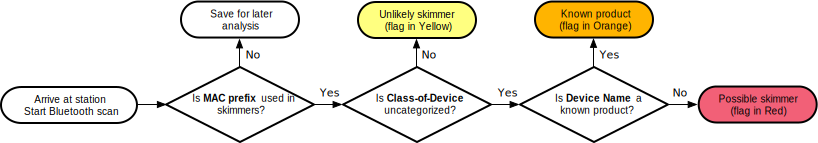
\includegraphics[width=\linewidth]{skimmer/fig/bluetana-flagging-flow}
  \caption{
  The procedure Bluetana uses for highlighting suspicious devices.
  %The MAC address of the device is first checked against a
  %hitlist of known skimming devices. Is this check succeeds, the Class-of-Device and
  %device name of the device are checked for innocuity. If these checks fail, the device
  %is flagged as a potential skimmer.
  \label{fig:bluetana-flagging-flow}
  }
  \end{figure}
  

This simple highlighting proved to be vital to our data collection.
%
Red serves as a cue to perform signal strength localization:
%
it directed our users to collect more samples of signal strength to determine
if a device is located in the gas pump area---and is therefore likely to
be a skimmer. 
%
In several cases, Bluetana highlighting a device in red was the only reason officials performed a manual skimmer inspections:
%
out of the \totalskimmers~skimmers we found, \Bluetanaskimmerfield~were recovered
because an official started an inspection only after noticing a device was highlighted in red in Bluetana.
%

In one instance, an Arizona Weights and Measures inspector was driving by a gas station when two red highlighted devices appeared in Bluetana.
%
He made an unscheduled stop at the gas station, performed a skimmer inspection, and discovered two skimmers.
%
Figure~\ref{fig:arizona_driveby} shows a portion of the official Arizona inspection report documenting this incident.

\begin{figure}[!h]
  \centering
  \captionsetup{justification=centering}
  \includegraphics[width=\textwidth,height=3cm]{skimmer/fig/arizona_driveby_anecdote.png}
  \caption{
  \label{fig:arizona_driveby}
 Bluetooth scanning helps inspectors find more skimmers because they detect skimmers when driving by a gas station.
  }
\end{figure}

Bluetana's highlighting procedure is more comprehensive than other skimmer detection apps on the Play Store.
%
Scaife et al. \cite{scaifeoakland} investigated the behavior of these apps and found that they flag skimmers based on either MAC prefix or Device Name.
%
These apps would miss skimmers with non-standard MAC prefixes or customized (missing) device names which Bluetana was able to find (Section~\ref{sec:bluetooth:skimmers}).
%
Bluetana also found legitimate devices that would be considered skimmers by these apps (Section~\ref{sec:bluetooth:scans}).

\begin{comment}  
As a result, the application accounts for the entire Bluetooth scan
response and is more comprehensive than any Bluetooth skimmer scanning
application available.
%
A rigorous study of Bluetooth-enabled skimmer detection applications was performed by Scaife et al.
\cite{scaifeoakland} and found majority of these applications look at only one feature
of the scan response packet (e.g. the MAC prefix).
\end{comment}

\subsubsection*{Identifying skimmers after data collection}
\label{sec:blu:identify}

\begin{figure}
\centering
\captionsetup{justification=centering}
\includegraphics[width=0.8\linewidth]{skimmer/fig/rssi_motivation.pdf}
\caption{
\label{fig:rssi}
  RSSI data overlaid on satellite view of a gas pump. Device on left has high RSSI near the gas pump and is likely a skimmer, device on the right is not. 
}
\end{figure}

During the study, we manually examined every Classic Bluetooth device observed
at a gas station visit in real time (as Bluetana users upload their scan data).
%
At the beginning of our study, we relied primarily on the signal strength of the device to determine if it was
a suspected skimmer.
%
By the nature of being installed inside a gas pump, the Bluetooth signal
of a skimmer is strongest in the pump area.
%
Other devices that we suspected to be skimmers all had a low signal strength
in the pump area, because aside from the cars parked at the pumps, the only
places where a Bluetooth device would be located in the pump area would be
inside the pump.
%
Combining the signal strength and geo-location with satellite
imagery of the gas station, we were able to easily detect when the signal was
emanating from inside of a gas pump (example shown in Figure~\ref{fig:rssi}).
%
While at a gas station, Bluetana users also noticed this by moving toward the
pump area to see if the device's signal strength increases.
%

If we saw any suspicious devices in the dataset, we alerted officials that they
should inspect the pumps at the station in question.
%
Initially, we did not know which of these devices were skimmers: many initial
inspections we requested turned up empty handed.
%
However, as the study progressed, we improved our understanding of the
profile of skimmers.

\subsubsection*{A natural experiment observing deployment duration}

Having a database of all prior scans made it possible
for us to look for skimmers that we may have missed in the past.
%
In particular, looking back in at the database led to us to discover two 
skimmers that we had initially missed.
%
A retroactive analysis of two stations discovered skimmers that were still
operating even though we first detected them \emph{six months} earlier.
%
This natural experiment is likely the first concrete data on how long skimmers
can be installed  without being found in a routine or complaint-induced pump inspection.
%
%%The two other skimmers were not seen on the second visit, but the station had
%%two pumps marked as inoperative\footnote{This is the typical behavior of
%station owners when they find skimmers in pumps}.


%}}}

\subsection{Limitations} %{{{

\subsubsection*{Selection bias}

We designed our data collection to look for a specific type of gas pump
skimmer: one that uses a Classic Bluetooth module, and is discoverable in
Bluetooth scans.
%
Our contacts in LE confirmed that this type of skimmer has been found in gas stations across
the entire U.S.
%
They also reported that these skimmers are particularly common in Arizona and California; therefore, these states were the focus of our study.
%
%Comparing our data collection with Arizona Weights and Measures reports, we
%find that in 2019 at least 60\% of the skimmers recovered in Arizona had
%classic, discoverable, Bluetooth modules.
  
The results of our study may not be representative of the nature of
gas pump skimming across the country.
%
Criminals in other regions may evade Bluetooth-based detection by using alternate exfiltration methods (e.g., Bluetooth Low
Energy and SMS), or configurations (e.g., non-discoverable mode).
%  
We outline these countermeasures in Section~\ref{sec:hiding}.

\subsubsection*{Bluetana does not connect to devices}
\label{sec:cant-connect}

We could collect more data about Bluetooth devices by trying to connect to
them.
%
This could be useful for conclusively detecting a skimmer or collecting information
about the type of Bluetooth device.
%
By sending commands that skimmers are known to respond to, Bluetana would be able to
see if the device responds equivalently to known skimmers. 
%
This is precisely what one of the current Bluetooth skimmer scanning applications on
the Play Store does.

This practice may seem innocuous, but our discussions with law enforcement
indicate that this could overwrite information critical to future
investigations.
%
The problem is, internal registers in many skimmer Bluetooth modules records the
last-paired MAC address.
%
This information can be used to link a suspect possessing a smartphone or
laptop with their skimmers.
%
The typical forensic evidence collection performed by law enforcement on
skimmers includes collecting the last-paired MAC address~\cite{swgdepractices}. 



%Also, our methodology does not apply to skimmers that use Bluetooth Low Energy (BLE)
%modules, or those that may employ countermeasures to avoid detection (e.g.,
%non-discoverable mode).
%
%It also does not apply to skimmers that use alternate wireless technologies 
%to exfiltrate card data (e.g., SMS).
%


%However, in our study we only survey four U.S. states.
%

%
%Alsoexfiltration technologies or may be popular in other states.

%}}}

%% \subsection{How does Bluetana compare to other skimmer detection applications?} %{{{
%% \label{sec:app-comparison}

\if 0 % extra text {{{
%
Unfortunately, many of these apps attempt to pair with the device, which as was
discussed earlier, is problematic for investigators\footnote{This is one of the
reasons we did not include the Service Discovery Protocol in our
fingerprinting}.

Bluetana is designed primarily to perform the large-scale measurement study
presented in this work. It is not intended as a tool that consumers can use to
detect skimmers. \noteby{MB}{Seems hypocritical given we just spent a whole section
  describing our methods of flagging devices Red.}
%
This is why it indiscriminately collects all the information possible from the
Android API.
%
In essence, Bluetana evaluates the heuristics used by other detection applications,
such as \emph{only} flagging devices that match a MAC Address prefix or device name of
recovered skimmers.
%
%Some apps do collect signal strength measurements and display this, but do not
%offer the live heat-map and correlation with gas station location that Bluetana
%is capable of.


This is particularly a problem at fuel stations, where Bluetooth scans are
likely to return legitimate devices; from auto entertainment systems, to
service station equipment.
%
In general, the presence Bluetooth devices at a fuel station is not an anomaly:
in 2017, it was projected that more than 5 billion Bluetooth devices would ship
out during the 2019 calendar year. ~\cite{bluetooth-popularity}.

The reason is, the firmware in the HC modules record the last paired MAC
address \todo{command?}. Therefore, any mechanism of detection should not
instantiate a serial connection, as it would interfere with the law enforcement. In order to work on the detection and prevention of skimming due to internally
process. In Android in particular, this also creates an issue with SPP lookup, installed devices, the features of the devices which are visible to an observer
as the \texttt{BluetoothDevice} method \texttt{fetchUuidsWithSdp}, which since must be described. Without specialized hardware, the data which is collectible
Android 6.0 has automatically triggered a pairing process with the device. A   about an internal skimmer is that which is exposed through the device's
more practical concern with SPP lookup is the additional time taken to perform Bluetooth interface \footnote{In this section, we address those portions of the
service discovery, a limitation which becomes important when adopting a        Bluetooth interface which are exposed while the device is in
crowd-sourced approach wherein the time spent scanning near the device may only\textit{discoverable} mode. Challenges and possibilities for handling
be on the order of 15 seconds with 20+ potential devices to perform service    non-discoverable mode are addressed in the discussion}. This interface includes
discovery on.                                                                  inquiry response meta-data from the device, serial port profiles (SPP)
accessible following initial connection, physical layer data such as signal
strength and location of observer, and possibly information which could be
exfiltrate by initiating a serial connection with the device and sending
commands or fuzzing input.

A CDF of discovery times may be seen in Figure~\ref{fig:skim_discover_time}










The Bluetana android application was developed as a method of crowd-sourced data collection on the Bluetooth environment, as well as a medium for real-time detection of skimmers. The application, which can run on standard consumer-grade cell phones, works by performing continuous enquiry scans and recording the responses received. The app allows for variable scan timing, ranging between 1 second and a full scan, which is on the range of 23 seconds, but somewhat hardware dependent. As results are received, they are highlighted red if they match any entries on a 'hit-list' of suspect Bluetooth modules. The application-level hit-list is more naive, relying on only simple metrics (manufacturer MAC address, Bluetooth type) to make the decision on whether a device is suspect or not. Once enough records have been received (3KB), the app uploads a csv of all the enquiry responses to a remote storage server hosted at UCSD. The records are stored in a Postgresql (PSQL) database for further analysis.

Once in the PSQL database, the records can be queried and more advanced analysis can take place. In order to determine what devices may be classified as suspicious, we developed a metric-based scoring system to isolate devices from within the data set. This set of metrics consists of flags which are set to one dependent on whether the device

\begin{enumerate}
\item \textbf{Is near a gas station:} the device is within 100 meters of a gas station.
\item \textbf{Is cheaply Available:} the manufacturer of the device is on a list of cheaply available Bluetooth boards.
\item \textbf{Has an Odd Name:} the devices name is in an outlier cluster, the methodology of which is described below.
\item \textbf{Is of an Uncategorized Device Type:} the devices type is labeled as 'uncategorized'.
\item \textbf{Has been Seen Twice:} the device was seen twice, with a time delta $>$ three hours between each observation.
\item \textbf{Is Non-BLE:} the device is non-Bluetooth Low Energy.
\end{enumerate}

These metrics are justified in the next section. Devices scoring high (flag set on all six metrics) are flagged and emailed to the research team as potential skimmers. All five of the skimmers found in this study scored $6/6$ on this set of metrics. The list of devices is rendered in a small web app and sorted in descending order based upon score in these metrics as well as the time last observed.

\todo{This section should describe the Bluetana app and data collection system, as well as how we determine what devices are suspicious.}
\fi
%}}}
